
\thesistitle{The Evolution of Marijuana Politics in the United States}

%"Dissertation" for PhD, "Thesis" for master's
\documenttitle{Dissertation}

\degreename{Doctor of Philosophy}

% Use the wording given in the official list of degrees awarded by UCI:
% http://www.rgs.uci.edu/grad/academic/degrees_offered.htm
\degreefield{Sociology}

% Your name as it appears on official UCI records.
\authorname{Burrel James Vann Jr}

% Use the full name of each committee member.
\committeechair{Edwin Amenta}
\othercommitteemembers
{
  David S. Meyer\\
  Charles Ragin\\
  Rory McVeigh
}

\degreeyear{2019}

\copyrightdeclaration
{
  {\copyright} {\Degreeyear} \Authorname
}

% If you have previously published parts of your manuscript, you must list the
% copyright holders; see Section 3.2 of the UCI Thesis and Dissertation Manual.
% Otherwise, this section may be omitted.
% \prepublishedcopyrightdeclaration
% {
% 	Chapter 4 {\copyright} 2003 Springer-Verlag \\
% 	Portion of Chapter 5 {\copyright} 1999 John Wiley \& Sons, Inc. \\
% 	All other materials {\copyright} {\Degreeyear} \Authorname
% }

% The dedication page is optional
% (comment out to exclude).
\dedications
{
  To my communities...
}

\acknowledgments
{
  I would like to thank numerous individuals and organizations, without whom this dissertation would not have been possible. 
  
  I am grateful to Edwin Amenta, whose advisement and steered the direction of this work. I am also thankful for David Meyer, who, even before graduate school was willing to help me devise good research projects, while also caring about my wellbeing. Finally, I would like to thank Rory McVeigh, whose guidance, advice, mentorship, and work has heavily influenced this work. 
  
  I would also like to thank faculty at the University of California, Irvine who have provided feedback and support along the way, including Evan Schofer, Nina Bandelj, Carter Butts, John Hipp, David Snow, Yang Su, Charles Ragin, Andrew Noymer, Sabrina Strings, Rocio Rosales, Jacob Avery, Katie Bolzendahl, and Katie Faust. In addition, I would like to thank the staff who've made my time at Irvine seamless, including John Sommerhauser, Ekua Arhin, Maryann Zovak-Wieder, and Hannah Absher.
  
  Of course, I cannot forget my UCI student life family. These people have been critical to my success and sanity during graduate school. I would like to thank Mart\'{i}n Jacinto, Miles Davison, Jess Lee, Sara Villalta, Claudia Campos, Alma Garza, Monique Kelly, Dana Moss, Thomas Elliott, Amber Tierney, Eulalie Laschever, Kara Placek, Ksenia Gracheva, Ted Watson, John McCollum, Bonnie Bui, Jessica Kizer, Connor Strobel, Chris Gibson, Aaron Tester, Katt Hoban, Steph Jones, Mariam Ashtiani, Alice Motes, Dana Nakano, Hector Y. Martinez, Matt Rafalow, Nolan Phillips, Jayson Hunt, and Tyson Patros. In addition, I would like to thank those amazing friends in my cohort: Emma Smith, Sean Drake, Tanya Sanabria, Chris Zoeller, Zaib Tufail, and David Kong. Importantly, my life would have not been the same without the intellect, wit, skills, and connections with my good friends Rodolfo Lopez and Ben Gibson. I am truly grateful for their friendship. 
  
  In 2011, I was lucky enough to conduct research at the University of Notre Dame. Over that Summer, and throughout the next year, I was able to develop strong relationships with many of my colleagues. Therefore, for their wisdom and friendship, I would like to thank Bryant Crubaugh,  San Diego-native Austin Choi-Fitzpatrick, (brother) Jeffrey Seymour, David Everson, Marshall Taylor, Kevin Estep, Heather Price, Peter Barwis, Kristi Donaldson, Jonathan Schwarz, Nicole Perez, Ana Velitchkova, Ellen Childs, Josh Dinsman, Amy Jonason, Jade Avelis, Linda Kawentel, Megan Rogers, Megan Austin, and Matthew Chandler. Most importantly, I am so appreciative of my dude... my co-metalcorehead/co-insert-subgenre-here-head/$\emptyset$ fam, Justin Van Ness. Over the years, we've crashed on each other's couches, gone to shows, explored cities, eaten good food, suggested new bands, tried out new breweries, and rocked tf out together, while being professional by presenting our work at conferences, networking, and crankin' papes. Cheers to keeping it strong for many years to come.
  
I am grateful for my Ford Foundation family, which has been integral to my success. I would like to thank 
  
  Music: I would like to give a shout out to all the musicians and artists whose work kept me motivated to complete this work.
  
  My Family:
  
  Unsung Family: 
  
  I would also like to thank the Ford Foundation for funding earlier versions of this project through the Predoctoral Fellowship and the Dissertation Fellowship. 
  
}


% Some custom commands for your list of publications and software.
%\newcommand{\mypubentry}[3]{
%  \begin{tabular*}{1\textwidth}{@{\extracolsep{\fill}}p{4.5in}r}
%    \textbf{#1} & \textbf{#2} \\ 
%    \multicolumn{2}{@{\extracolsep{\fill}}p{.95\textwidth}}{#3}\vspace{6pt} \\
%  \end{tabular*}
%}
%\newcommand{\mysoftentry}[3]{
%  \begin{tabular*}{1\textwidth}{@{\extracolsep{\fill}}lr}
%    \textbf{#1} & \url{#2} \\
%    \multicolumn{2}{@{\extracolsep{\fill}}p{.95\textwidth}}
%    {\emph{#3}}\vspace{-6pt} \\
%  \end{tabular*}
%}

% Include, at minimum, a listing of your degrees and educational
% achievements with dates and the school where the degrees were
% earned. This should include the degree currently being
% attained. Other than that it's mostly up to you what to include here
% and how to format it, below is just an example.
%
% CV is required for PhD theses, but not Master's
% comment out to exclude
\curriculumvitae
{
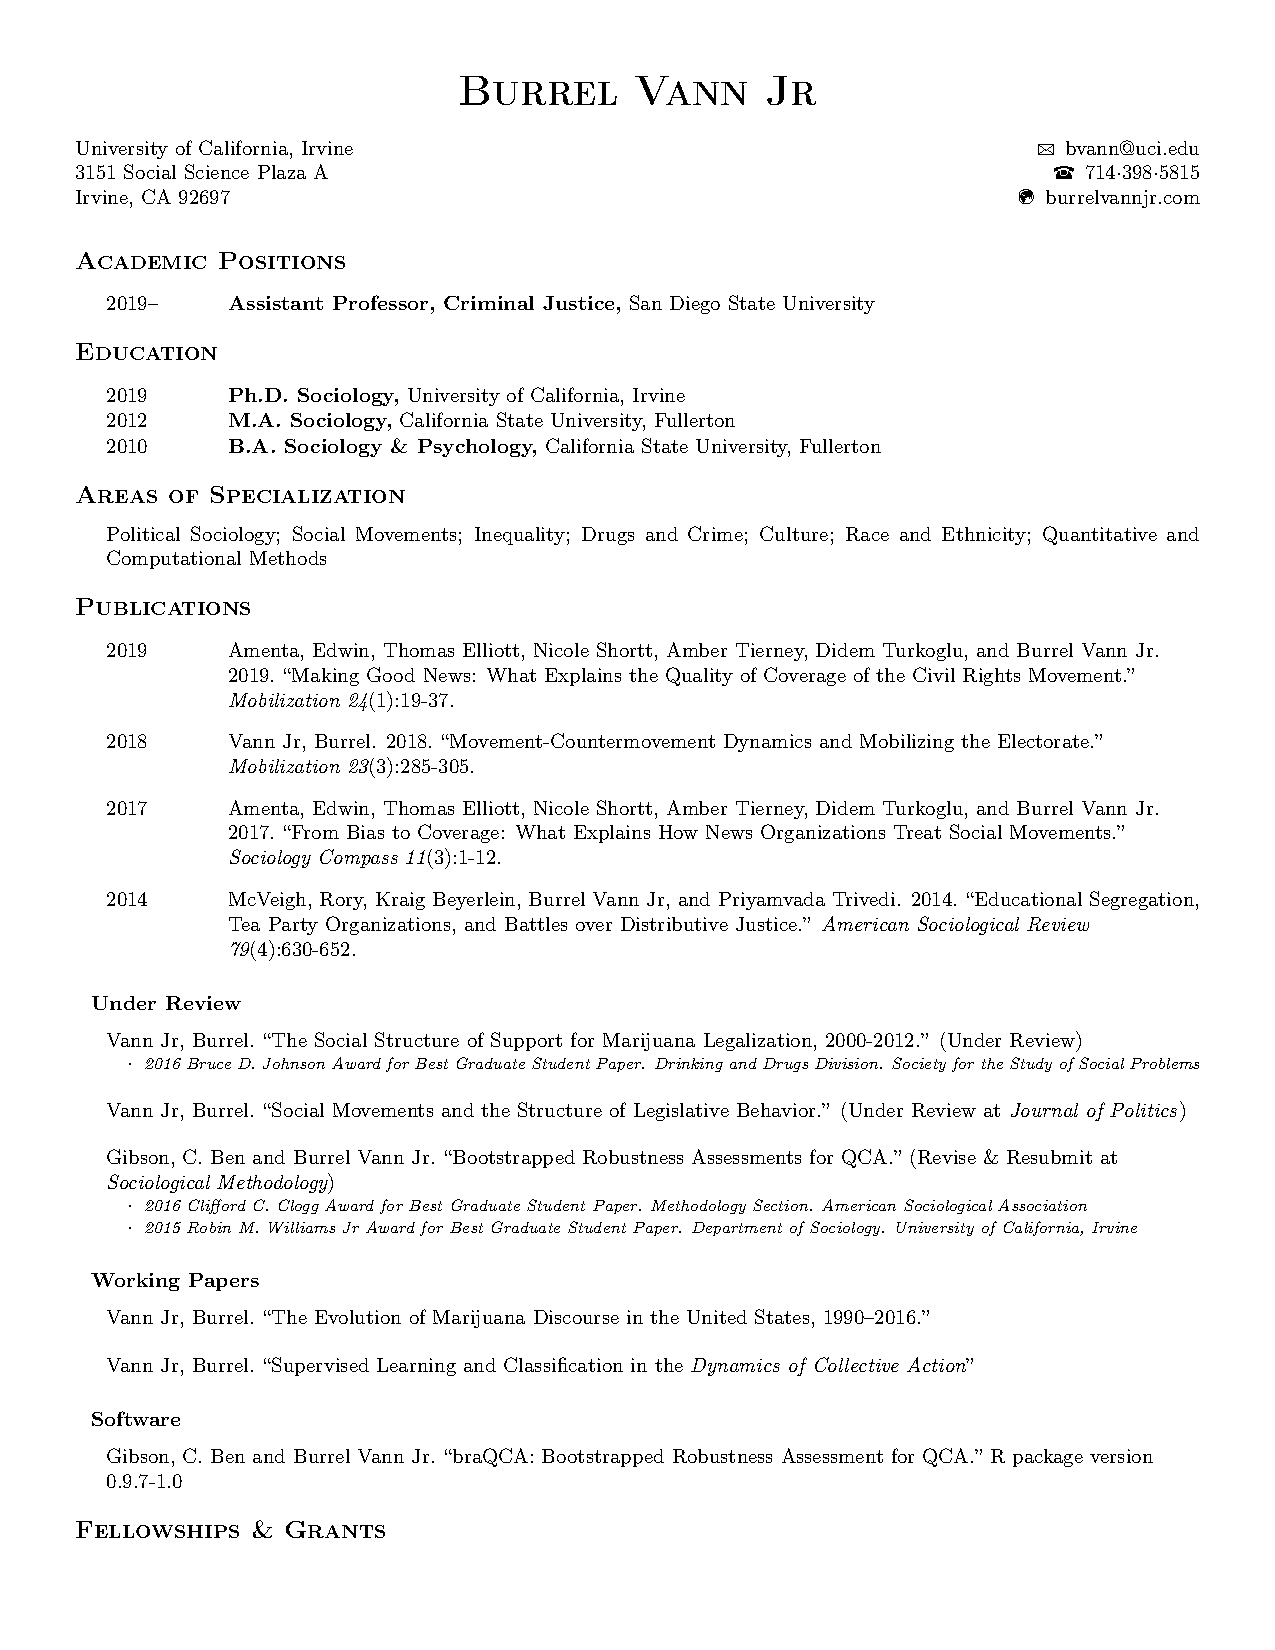
\includepdf[pages=-,pagecommand={}]{cv.pdf}
%\textbf{EDUCATION}
  
%  \begin{tabular*}{1\textwidth}{@{\extracolsep{\fill}}lr}
%    \textbf{Doctor of Philosophy in Computer Science} & \textbf{2012} \\
%    \vspace{6pt}
%    University name & \emph{City, State} \\
%    \textbf{Bachelor of Science in Computational Sciences} & \textbf{2007} \\
%    \vspace{6pt}
%    Another university name & \emph{City, State} \\
%  \end{tabular*}

%\vspace{12pt}
%\textbf{RESEARCH EXPERIENCE}

%  \begin{tabular*}{1\textwidth}{@{\extracolsep{\fill}}lr}
%    \textbf{Graduate Research Assistant} & \textbf{2007--2012} \\
%    \vspace{6pt}
%    University of California, Irvine & \emph{Irvine, California} \\
%  \end{tabular*}

%\vspace{12pt}
%\textbf{TEACHING EXPERIENCE}

%  \begin{tabular*}{1\textwidth}{@{\extracolsep{\fill}}lr}
%    \textbf{Teaching Assistant} & \textbf{2009--2010} \\
%    \vspace{6pt}
%    University name & \emph{City, State} \\
%  \end{tabular*}

%\pagebreak

%\textbf{REFEREED JOURNAL PUBLICATIONS}

%  \mypubentry{Ground-breaking article}{2012}{Journal name}

%\vspace{12pt}
%\textbf{REFEREED CONFERENCE PUBLICATIONS}

%  \mypubentry{Awesome paper}{Jun 2011}{Conference name}
%  \mypubentry{Another awesome paper}{Aug 2012}{Conference name}

%\vspace{12pt}
%\textbf{SOFTWARE}

%  \mysoftentry{Magical tool}{http://your.url.here/}
%  {C++ algorithm that solves TSP in polynomial time.}

}




%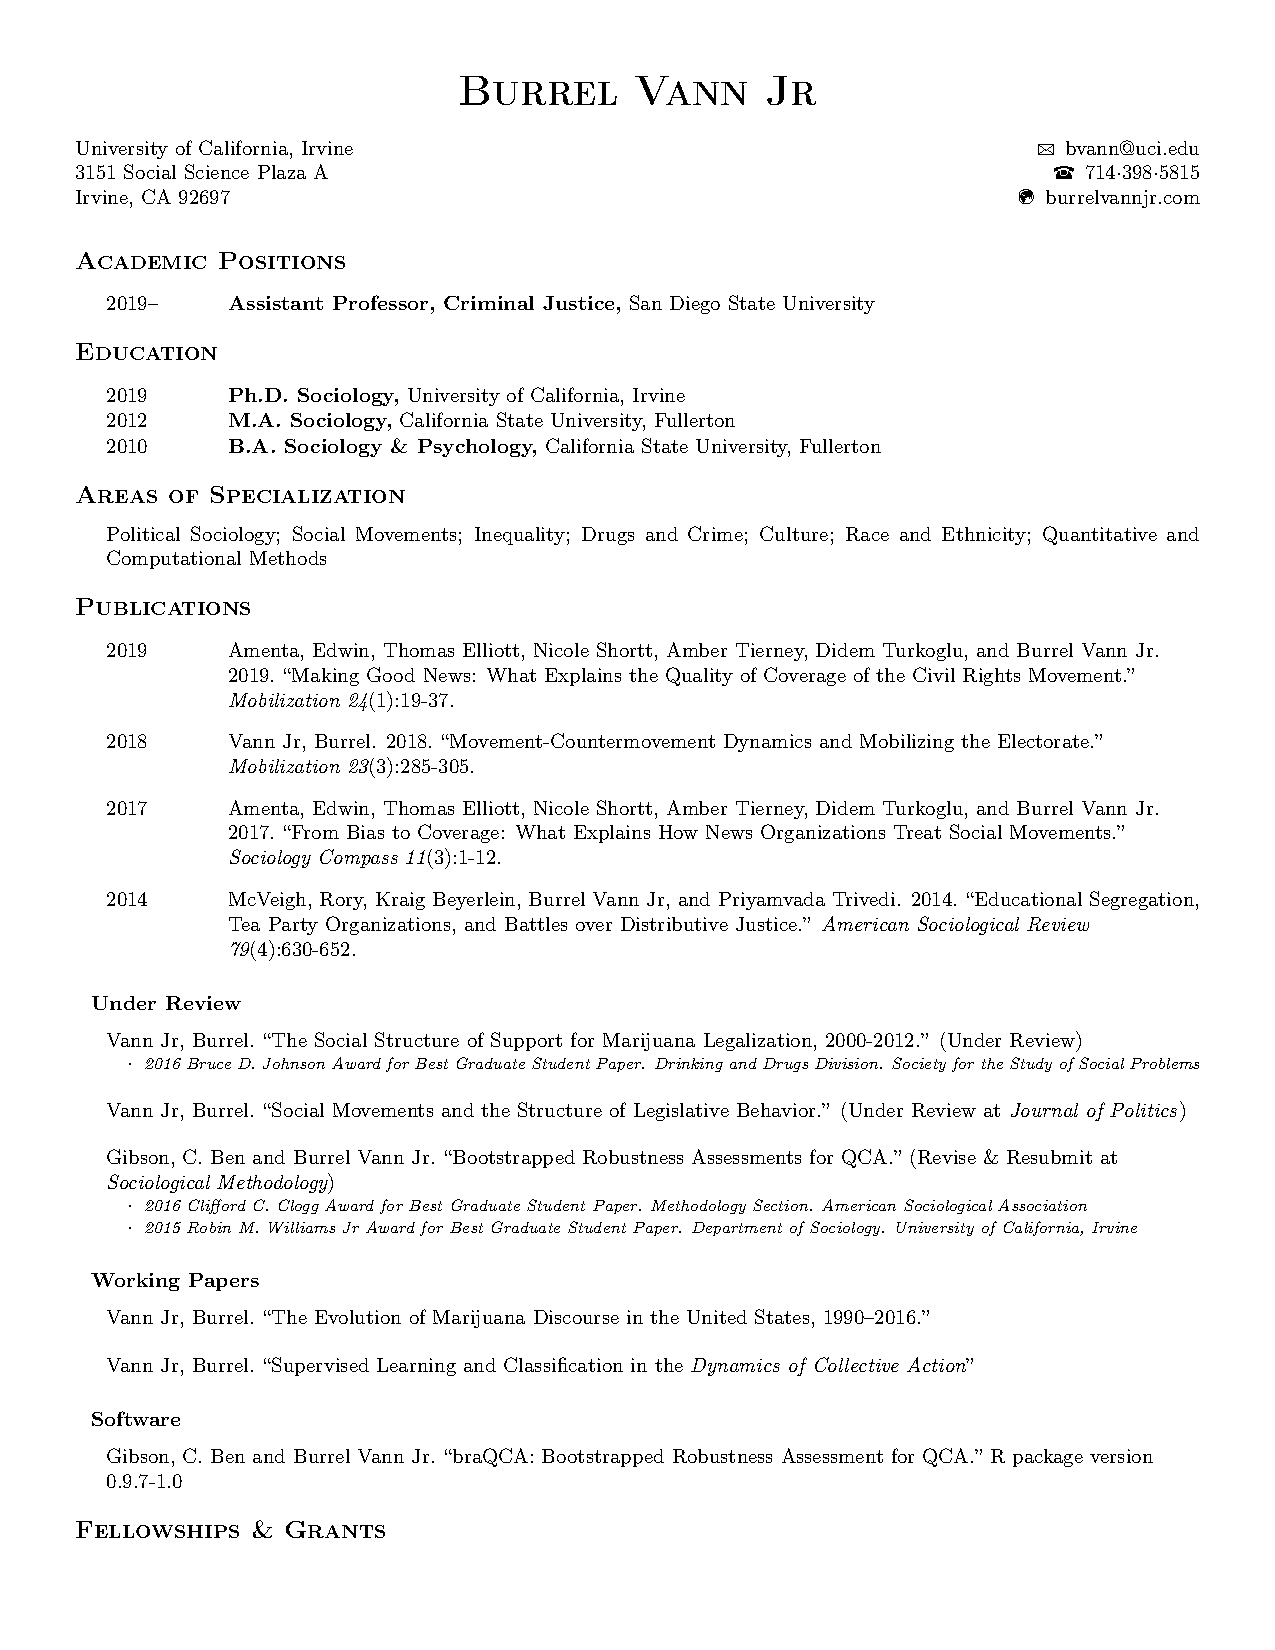
\includepdf[pages=1-]{cv.pdf}

% The abstract was previously limited to a maximum of 350 words, 
% but the UCI manual at https://etd.lib.uci.edu/electronic/td2e#2.2.1.
% currently does not indicate that there is any word limit for the abstract
\thesisabstract
{
  The abstract of your contribution goes here.
}


%%% Local Variables: ***
%%% mode: latex ***
%%% TeX-master: "thesis.tex" ***
%%% End: ***
